%!TEX root = ClementiCooperBarba2018.tex

\subsection{Verification against analytical solution} \label{sec:verification}

We need to run convergence on single sphere of radius 8nm

Plot of verification

\begin{figure}[h] %  figure placement: here, top, bottom, or page
   \centering
   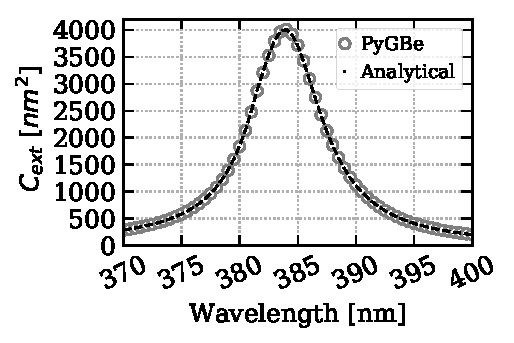
\includegraphics[width=0.4\textwidth]{silver_NP_verification.pdf} 
   \caption{Verification}
   \label{fig:verif_sphere}
\end{figure}

\subsection{Silver nanoparticle response to BSA} \label{sec:verification}

Put diagram of system

Convergence analysis for system sensor-BSA


\begin{figure}[h] %  figure placement: here, top, bottom, or page
   \centering
   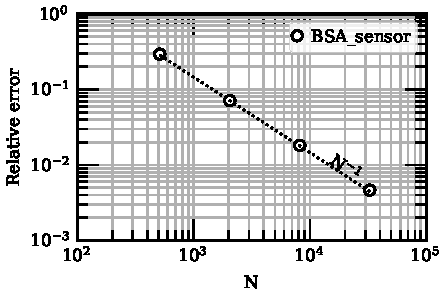
\includegraphics[width=0.4\textwidth]{convergence_bsa_sensor_R8_d=1_w=380.pdf} 
   \caption{Grid-convergence study for the silver spherical nanoparticle response to Bovine Serum Albumina (BSA). We performed
            the mesh-refinement on the sensor (silver nanoparticle) since this is the surface where the extinction cross section 
            is computed. We run the case presented in (insert ref to diagram figure) for radius of the sphere of 8nm, a wavelength
            of  380 nm and a distance d=1nm along the z-axis, for sensor-meshes of 512, 2048, 8192 and 32768 elements. The error 
            calculation uses the Richardson extrapolation value of the extinction cross section as a reference $C_{ext} = 1778.7259 \; nm^2$, 
            computed using the 3 finner meshes.}
   \label{fig:error_sphere-bsa}
\end{figure}


We can see in Figure \ref{fig:error_sphere-bsa} the error decays with number of boundary elements ($\frac{1}{N}$), which is consistent with our verification 
results (reference verification convergence figure). This proves that the numerical solutions computed with \pygbe are correctly resolved by the meshes. 


Put fig of 2pz visualization

Fig result of 2pz

Put fig of 2px and 2py visualization

Fig result of 2px and 2py

